\documentclass[
	a4paper,
	oneside,
	DIV = 12,
	fontsize = 13pt,
	headings = normal,
]{scrartcl}

%%% Page geometry and precise margins
\usepackage[
	pass,
	left   = 20mm,
	top    = 15mm,
	right  = 10mm,
	bottom = 15mm,
]{geometry}
%%%

%%% Length calculations
\usepackage{calc}
%%%

%%% Support for color
\usepackage{xcolor}
\definecolor{lightblue}{HTML}{03A9F4}
\definecolor{red}{HTML}{F44336}
%%%

%%% Including graphics
\usepackage{graphicx}
%%%

%%% Font selection
\usepackage{fontspec}

\setromanfont{STIX Two Text}[
	SmallCapsFeatures = {LetterSpace = 5},
]

\setsansfont{IBM Plex Sans}[
	Scale = MatchUppercase,
]

\setmonofont{IBM Plex Mono}[
	Scale = MatchUppercase,
]
%%%

%%% Math typesetting
\usepackage{amsmath}

\usepackage{unicode-math}
\setmathfont{STIX Two Math}
%%%

%%% List settings
\usepackage{enumitem}
\setlist[enumerate]{
	label*      = {\arabic*.},
	leftmargin  = *,
	labelindent = \parindent,
	topsep      = 1\baselineskip,
	parsep      = 0\baselineskip,
	itemsep     = 1\baselineskip,
}

\setlist[itemize]{
	label       = {—},
	leftmargin  = *,
	labelindent = \parindent,
	topsep      = 1\baselineskip,
	parsep      = 0\baselineskip,
	itemsep     = 1\baselineskip,
}

\setlist[description]{
	font        = {\rmfamily\upshape\bfseries},
	topsep      = 1\baselineskip,
	parsep      = 0\baselineskip,
	itemsep     = 0\baselineskip,
}

%%%

%%% Structural elements typesetting
\setkomafont{pagenumber}{\rmfamily}
\setkomafont{disposition}{\rmfamily\bfseries}

% Sectioning
\RedeclareSectionCommand[
	beforeskip = -1\baselineskip,
	afterskip  = 1\baselineskip,
	font       = {\normalsize\bfseries\scshape},
]{section}

\RedeclareSectionCommand[
	beforeskip = -1\baselineskip,
	afterskip  = 1\baselineskip,
	font       = {\normalsize\bfseries},
]{subsection}

\RedeclareSectionCommand[
	beforeskip = -1\baselineskip,
	afterskip  = 1\baselineskip,
	font       = {\normalsize\bfseries},
]{subsubsection}
%%%

%%% Typographic enhancements
\usepackage{microtype}
%%%

%%% Language-specific settings
\usepackage{polyglossia}
\setmainlanguage{ukrainian}
\setotherlanguages{english, russian}
%%%

%%% Captions
\usepackage{caption}
\usepackage{subcaption}

%\DeclareCaptionLabelFormat{closing}{#2)}
%\captionsetup[subtable]{labelformat = closing}

%\captionsetup[subfigure]{labelformat = closing}

\captionsetup[table]{
	aboveskip = 0\baselineskip,
	belowskip = 1\baselineskip,
}

\captionsetup[figure]{
	aboveskip = 1\baselineskip,
	belowskip = 0\baselineskip,
}

\captionsetup[subfigure]{
	aboveskip = 0.25\baselineskip,
	belowskip = 0\baselineskip,
}

\captionsetup[subfigure]{
	labelformat = simple,
	labelformat = brace,
}
%%%

%%% Table typesetting
\usepackage{booktabs}
\usepackage{longtable}

\usepackage{multirow}

\usepackage{array}
\newcolumntype{v}[1]{>{\raggedright\arraybackslash\hspace{0pt}}p{#1}}
\newcolumntype{b}[1]{>{\centering\arraybackslash\hspace{0pt}}p{#1}}
\newcolumntype{n}[1]{>{\raggedleft\arraybackslash\hspace{0pt}}p{#1}}
%%%

%%% Dingbats
\usepackage{pifont}
%%%

%%% TikZ
\usepackage{tikz}
%%%

%%% Links and hyperreferences
\usepackage{hyperref}
\hypersetup{
	bookmarksnumbered = true,
	colorlinks      = false,
	linkbordercolor = red,
	urlbordercolor  = lightblue,
	pdfborderstyle  = {/S/U/W 1.5},
}
%%%

%%% Length adjustments
% Set baselineskip to ~15pt, default is 14.5pt
% \linespread{1.034483}
% \linespread{1.068966} % ~15.5pt
\setlength{\emergencystretch}{1em}
\setlength{\parindent}{1.5em}
\newlength{\gridunitwidth}
\setlength{\gridunitwidth}{\textwidth / 12}
\setlength{\floatsep}{1\baselineskip}
\setlength{\intextsep}{1\baselineskip}
\setlength{\textfloatsep}{1\baselineskip}
%%%

%%% Custom commands
\newcommand{\allcaps}[1]{{\addfontfeatures{LetterSpace = 5}#1}}
\newcommand{\progname}[1]{\texttt{#1}}

\newcommand{\CheckMark}{\ding{51}}
\newcommand{\Mytextrightarrow}{$\rightarrow$\hspace{0.25em}}

\newcommand{\filename}[1]{\texttt{#1}}
%%%

%%% Make typography adhere to made-up standards
\PolyglossiaSetup{ukrainian}{indentfirst = true}

% Sectioning
\RedeclareSectionCommand[
	beforeskip = -0sp,
	afterskip  = 1sp,
	indent     = 12.5mm,
	font       = {\normalsize\bfseries},
]{section}

\RedeclareSectionCommand[
	beforeskip = -0sp,
	afterskip  = 1sp,
	indent     = 12.5mm,
	font       = {\normalsize\bfseries},
]{subsection}

\RedeclareSectionCommand[
	beforeskip = -0sp,
	afterskip  = 1sp,
	indent     = 12.5mm,
	font       = {\normalsize\bfseries},
]{subsubsection}

\setlength{\parindent}{12.5mm}

\usepackage{leading}
\leading{21pt}


\captionsetup[table]{
	aboveskip = 0\baselineskip,
	belowskip = 0.25\baselineskip,
}

\captionsetup[figure]{
	aboveskip = 0.25\baselineskip,
	belowskip = 0\baselineskip,
}

\captionsetup[subfigure]{
	aboveskip = 0.25\baselineskip,
	belowskip = 0\baselineskip,
}

\captionsetup[subfigure]{
	labelformat = simple,
	labelformat = brace,
}

%%%

\begin{document}
	\newgeometry{
		left   = 20mm,
		top    = 15mm,
		right  = 10mm,
		bottom = 15mm,
		footskip = \baselineskip, % reduce footer vertical skip so page numbers are visible
	}
\setlength{\gridunitwidth}{\textwidth / 12}
	\begin{titlepage}
		\begin{center}
			Міністерство освіти і науки України\\
			Національний авіаційний університет\\
			Навчально-науковий інститут комп'ютерних інформаційних технологій\\
			Кафедра комп'ютеризованих систем управління

			\vspace{\fill}
				Лабораторна робота №8\\
				з~дисципліни «Діагностика та~експлуатація комп'ютера»\\
				на~тему «Адміністрування ОС \textenglish{Windows}»\\

			\vspace{\fill}

			\begin{flushright}
				Виконав:\\
				студент \allcaps{ННІКІТ}\\
				групи СП-325\\
				Клокун В.\,Д.\\
				Перевірив:\\
				Масловський Б.\,Г.
			\end{flushright}

			Київ 2018
		\end{center}
	\end{titlepage}

	\section{Ціль роботи}
		Отримати навички адміністрування в операційній системі~\textenglish{Windows 7}.

	% \section{Короткі теоретичні відомості}

	\section{Хід роботи}
		\subsection{Створення облікового запису користувача}
			Відкриваємо Панель керування, переходимо в меню «Адміністрування» та запускаємо оснащення «Управління комп'ютером». Відкриваємо значок «Службові програми» і вибираємо «Локальні користувачі та групи». Клікаємо на «Користувачі» правою кнопкою миші і вибираємо пункт «Новий користувач». Задаємо ім'я користувача та його пароль входу до системи. Натискаємо кнопку «Створити»~(рис.~\ref{fig:user-account-creation-dialog}).

			\begin{figure}[!htbp]
				\centering
				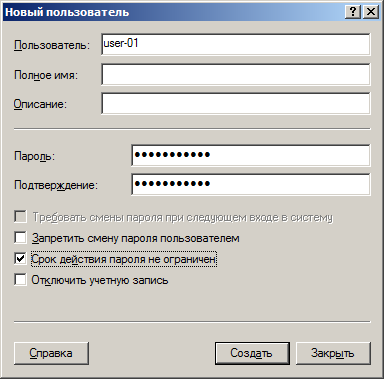
\includegraphics[height = 9\baselineskip]{../01-solution/y03s01-pcdiag-lab-08-p02.png}
				\caption{Вікно створення нового користувача}
				\label{fig:user-account-creation-dialog}
			\end{figure}%

			В результаті був створений новий обліковий запис користувача~(рис.~\ref{fig:user-account-creation-result}).

			\begin{figure}[!htbp]
				\centering
				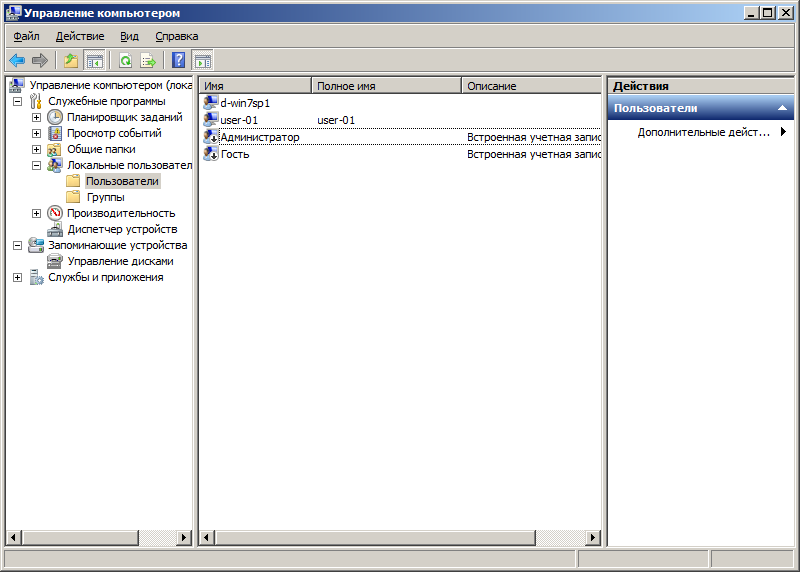
\includegraphics[height = 12\baselineskip]{../01-solution/y03s01-pcdiag-lab-08-p03.png}
				\caption{Результат створення нового користувача}
				\label{fig:user-account-creation-result}
			\end{figure}%

		%\begin{figure}[!htbp]
		%	\centering
		%	\begin{subfigure}[t]{0.4\columnwidth}
		%		\centering
		%		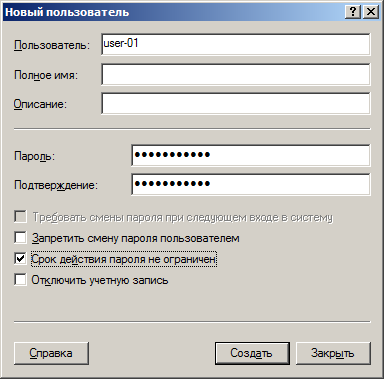
\includegraphics[height = 8\baselineskip]{../01-solution/y03s01-pcdiag-lab-08-p02.png}
		%		\caption{}
		%		\label{subfig:user-account-creation-dialog}
		%	\end{subfigure}%
		%	\begin{subfigure}[t]{0.6\columnwidth}
		%		\centering
		%		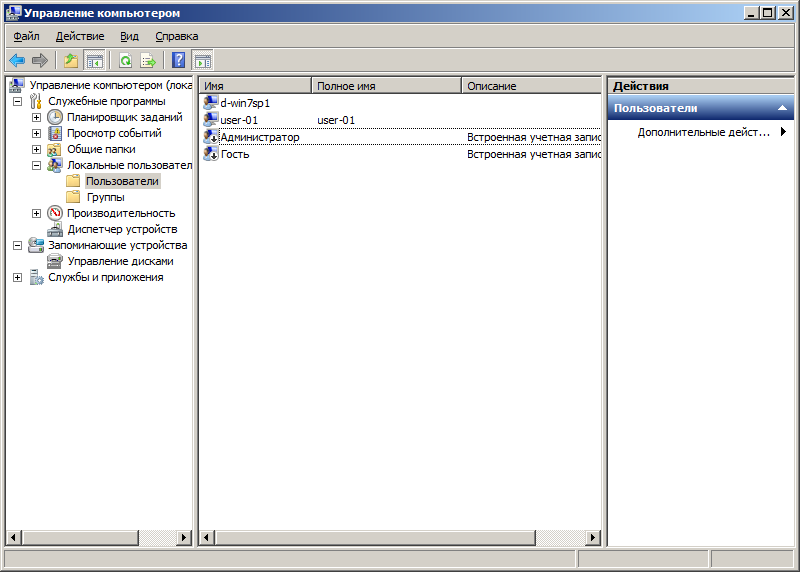
\includegraphics[height = 9\baselineskip]{../01-solution/y03s01-pcdiag-lab-08-p03.png}
		%		\caption{}
		%		\label{subfig:user-account-creation-result}
		%	\end{subfigure}%
		%	\caption{Створення облікового запису користувача}
		%	\label{fig:user-account-creation}
		%\end{figure}

		\subsection{Налаштування оточення користувача}
			Клікаємо на імені користувача правою кнопкою миші та обираємо «Властивості». На закладці «Членство в групах» виключаємо приналежність користувача до групи «Користувачі»~(рис.~\ref{fig:user-environment-setting}).

			\begin{figure}[!htbp]
				\centering
				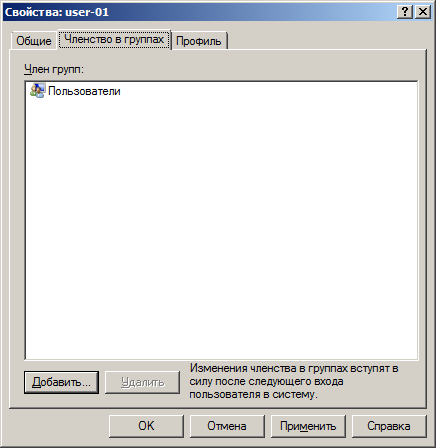
\includegraphics[height = 11.5\baselineskip]{../01-solution/y03s01-pcdiag-lab-08-p04-01.png}
				\caption{Належність нового користувача групам}
				\label{fig:user-environment-setting}
			\end{figure}

			В результаті новий користувач був доданий до групи «Користувачі».

		\subsection{Встановлення домашнього каталогу користувача}
			На закладці «Профіль» вказуємо шлях до папки, де будуть зберігатись індивідуальні файли користувача~(рис.~\ref{fig:home-folder}). 
			
			\begin{figure}[!htbp]
				\centering
				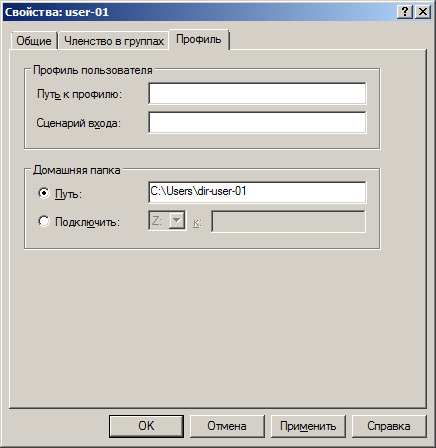
\includegraphics[height = 11.5\baselineskip]{../01-solution/y03s01-pcdiag-lab-08-p05.png}
				\caption{Встановлення шляху до домашньої папки користувача}
				\label{fig:home-folder}
			\end{figure}
			
			Створюємо свою групу користувачів~(рис.~\ref{fig:group-creation}).

			\begin{figure}[!htbp]
				\centering
				\begin{subfigure}[t]{0.4\columnwidth}
					\centering
					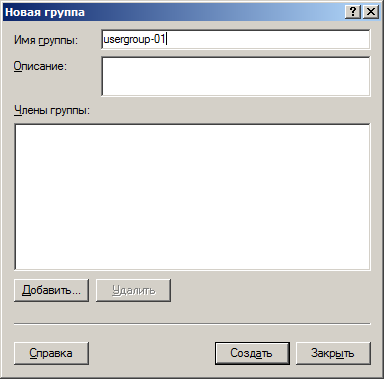
\includegraphics[width = \columnwidth - 1em]{../01-solution/y03s01-pcdiag-lab-08-p06.png}
					\caption{}
					\label{subfig:group-creation-dialog}
				\end{subfigure}%
				\begin{subfigure}[t]{0.6\columnwidth}
					\centering
					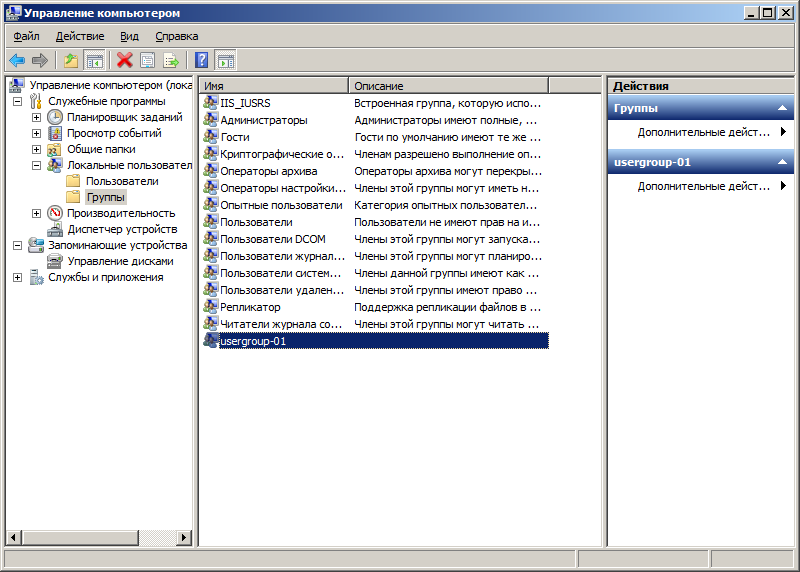
\includegraphics[width = \columnwidth]{../01-solution/y03s01-pcdiag-lab-08-p07.png}
					\caption{}
					\label{subfig:group-creation-result}
				\end{subfigure}%
				\caption{Створення нової групи користувачів}
				\label{fig:group-creation}
			\end{figure}

			В результаті була створена нова група користувачів.

		\subsection{Призначення прав користувачам і групам}
			В оснащенні «Адміністрування» вибираємо «Локальна політика безпеки» \Mytextrightarrow «Локальні політики» \Mytextrightarrow «Призначення прав користувача». Знаходимо право «Локальний вхід в систему» і обираємо меню «Безпека». Надаємо користувачу це право~(рис.~\ref{fig:user-rights-assignment}).

			\begin{figure}[!htbp]
				\begin{subfigure}[t]{0.5\columnwidth}
					\centering
					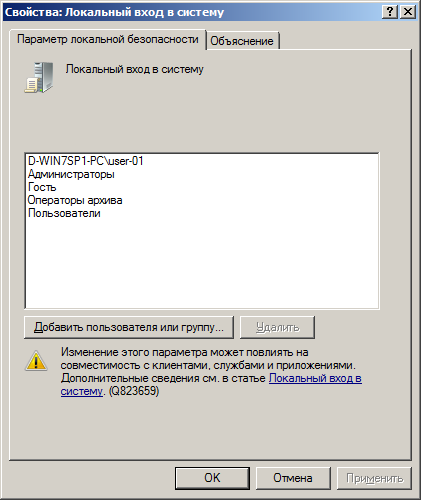
\includegraphics[height = 11\baselineskip]{../01-solution/y03s01-pcdiag-lab-08-p09.png}
					\caption{}
					\label{}
				\end{subfigure}%
				\begin{subfigure}[t]{0.5\columnwidth}
					\centering
					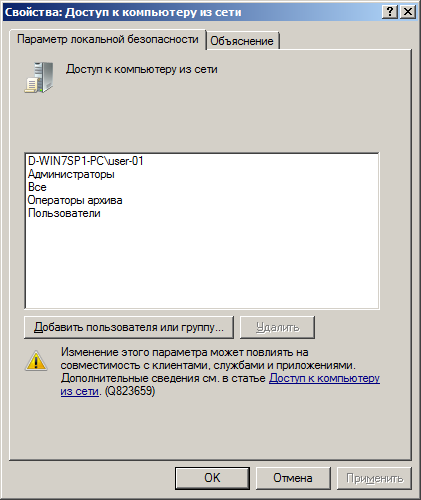
\includegraphics[height = 11\baselineskip]{../01-solution/y03s01-pcdiag-lab-08-p10.png}
					\caption{}
					\label{}
				\end{subfigure}%
				\caption{Встановлення дозволу на права «Локальний вхід в систему» і~«Доступ до комп'ютера з мережі» нашому користувачу}
				\label{fig:user-rights-assignment}
			\end{figure}

			Перевіряємо локальний вхід користувача на комп'ютер. Для цього завершуємо поточний сеанс і намагаємось зареєструватись під ім'ям користувача. Коли у користувача відсутнє право локального входу, його обліковий запис не з'являється у списку користувачів, які могуть входити в систему. Якщо у користувача є таке право, кнопка входу в систему стає доступною~(рис.~\ref{fig:logon-attempt}).

			\begin{figure}[!htbp]
				\begin{subfigure}[t]{0.5\columnwidth}
					\centering
					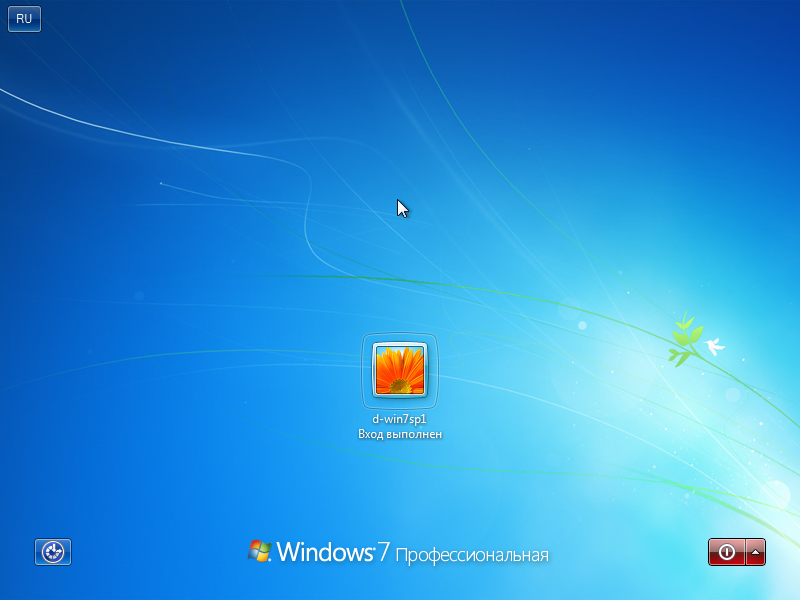
\includegraphics[height = 7\baselineskip]{../01-solution/y03s01-pcdiag-lab-08-p11-00.png}
					\caption{}
					\label{subfig:logon-attempt-access-denied}
				\end{subfigure}%
				\begin{subfigure}[t]{0.5\columnwidth}
					\centering
					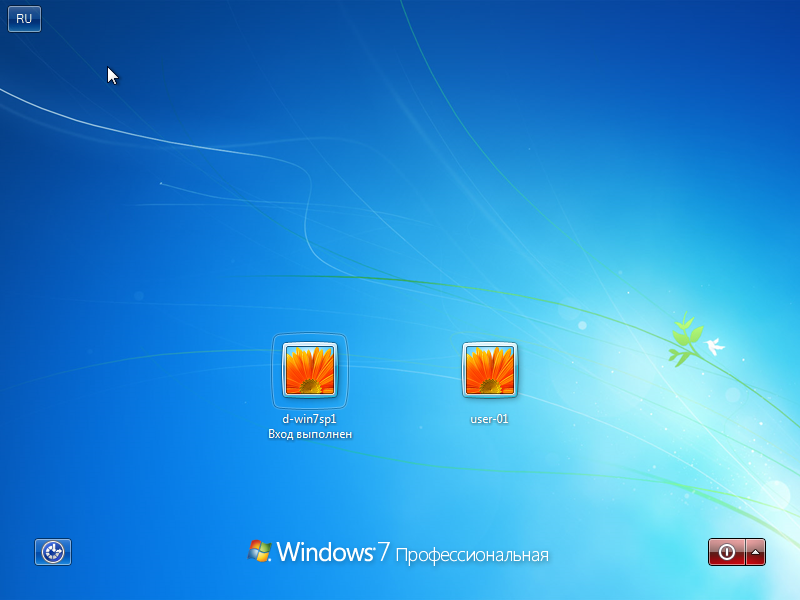
\includegraphics[height = 7\baselineskip]{../01-solution/y03s01-pcdiag-lab-08-p11-01.png}
					\caption{}
					\label{subfig:logon-attempt-access-granted}
				\end{subfigure}%
				\caption{Спроби входу в систему: \subref{subfig:logon-attempt-access-denied}~— якщо право відсутнє, \subref{subfig:logon-attempt-access-granted}~— якщо право надане}
				\label{fig:logon-attempt}
			\end{figure}

			В результаті ми призначили користувачу необхідні права.

		\subsection{Створення папки «\textenglish{Test}»}
			Створюємо на диску «\textenglish{C:}» папку «\textenglish{Test}» та налаштовуємо дозволи для цієї папки. Для цього клацаємо на ній правою кнопкою миші і відкриваємо «Властивості». Відкриваємо вкладку «Безпека» та визначаємо користувачів та дозволи, які вони мають на папку.

			Створюємо ще 3 користувача. В безпеці папки~«\textenglish{Test}» користувачу~1 надаємо дозвіл тільки на читання цієї папки, другому~— на читання і зміну, третьому~— повний доступ, четвертому~— забороняємо доступ~(рис.~\ref{fig:created-user-rights}).

			\begin{figure}[!htbp]
				\centering
				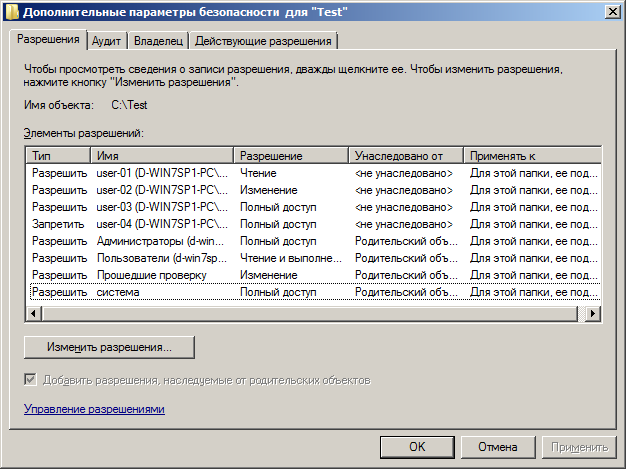
\includegraphics[height = 9\baselineskip]{../01-solution/y03s01-pcdiag-lab-08-p12.png}
				\caption{Створені права}
				\label{fig:created-user-rights}
			\end{figure}

			Реєструємося на машині послідовно під різними іменами та намагаємось створювати, змінювати і видаляти файли і папки всередині папки~«\textenglish{Test}». При виконанні операцій, на які користувач не має права, з'являється відповідне вікно з проханням ввести пароль адміністратора~(рис.~\ref{fig:user-access-prompt}).

			\begin{figure}[!htbp]
				\centering
				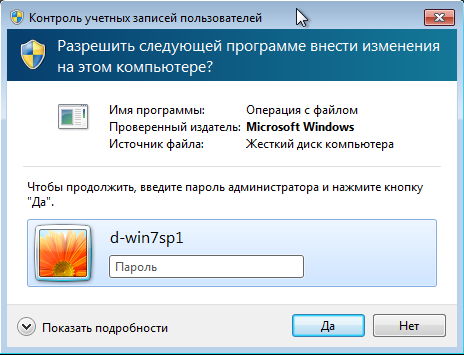
\includegraphics[height = 10\baselineskip]{../01-solution/y03s01-pcdiag-lab-08-p13-01.png}
				\caption{Вікно попередження}
				\label{fig:user-access-prompt}
			\end{figure}

		\subsection{Створення папки~«\textenglish{Test}» загальним (мережевим) ресурсом}
			Відкриваємо властивості папки~«\textenglish{Test}» і вибираємо закладку «Доступ». Відкриваємо загальний доступ до цієї папки і, клікнувши на кнопці «Дозволи», визначаємо можливості доступу до папки різних користувачів~(рис.~\ref{fig:test-dir-permissions}).

			\begin{figure}[!htbp]
				\centering
				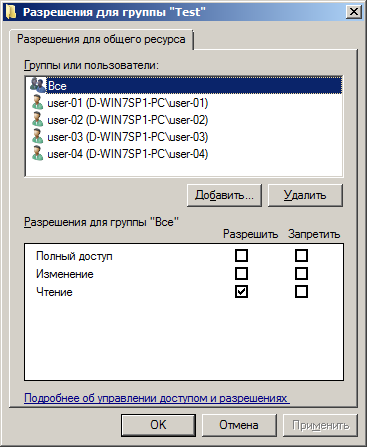
\includegraphics[height = 13\baselineskip]{../01-solution/y03s01-pcdiag-lab-08-p14.png}
				\caption{Створені дозволи для папки~«\textenglish{Test}»}
				\label{fig:test-dir-permissions}
			\end{figure}

		\subsection{Створення файлу у папці~«\textenglish{Test}»}
			Реєструємось на комп'ютері під ім'ям користувача~«\textenglish{user-03}», створюємо файл~«\textenglish{test-file}» та переконуємось, що цей користувач є його власником~(рис.~\ref{fig:test-file-owner}).

			\begin{figure}[!htbp]
				\centering
				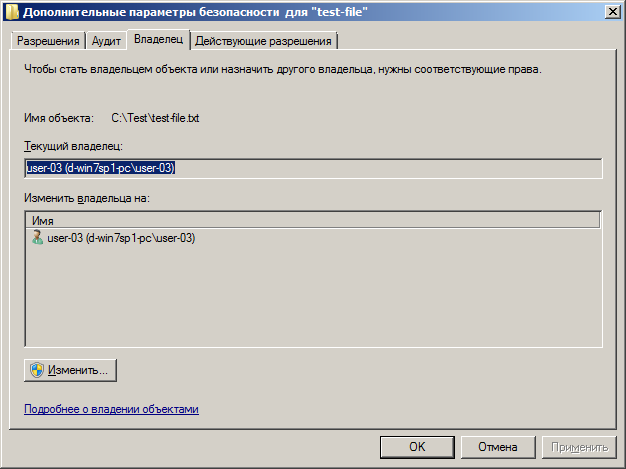
\includegraphics[height = 12\baselineskip]{../01-solution/y03s01-pcdiag-lab-08-p16.png}
				\caption{Інформація про власника файлу~«\textenglish{test-file}»}
				\label{fig:test-file-owner}
			\end{figure}

		\subsection{Встановлення і налаштування аудиту}
			Відкриваємо оснастку «Локальні політики» \Mytextrightarrow «Політика аудиту». Вибираємо пункт «Аудит доступу до об'єктів» і двічі клікаємо на ньому. У діалозі вибираємо «Відмова» та натискаємо «ОК»~(рис.~\ref{fig:audit-enabled}).

			\begin{figure}[!htbp]
				\centering
				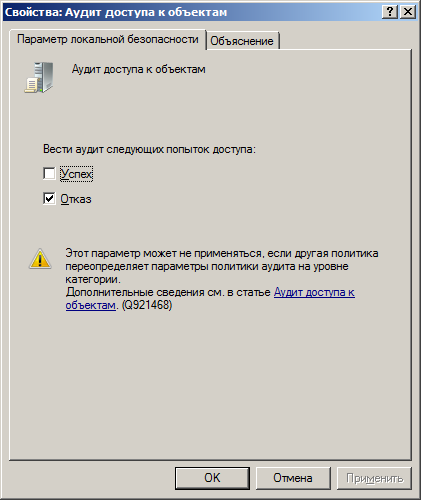
\includegraphics[height = 12\baselineskip]{../01-solution/y03s01-pcdiag-lab-08-p17.png}
				\caption{Увімкнення аудиту відмов}
				\label{fig:audit-enabled}
			\end{figure}

			Відкриваємо властивості папки~«\textenglish{Test}», закладку «Безпека» і натискаємо кнопку «Додатково». У діалозі вибираємо закладку «Аудит». Заносимо у список імена користувача, події аудиту якого будуть відслідковуватись. Додаємо до цього списку користувача, який не має дозволу на видалення файлу за папки~«\textenglish{Test}»~(рис.~\ref{fig:dir-audit-enabled}).

			\begin{figure}[!htbp]
				\centering
				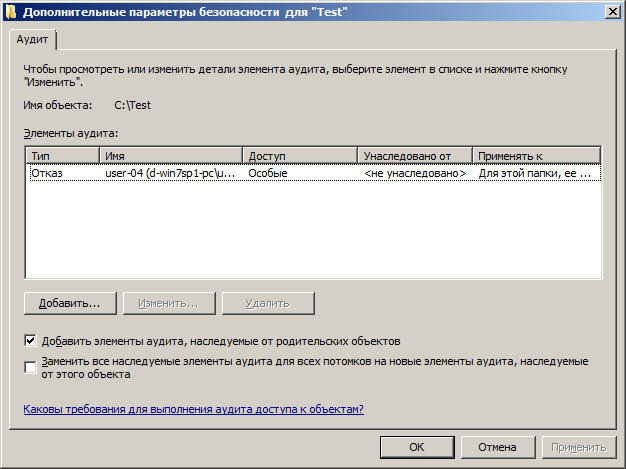
\includegraphics[height = 14\baselineskip]{../01-solution/y03s01-pcdiag-lab-08-p18.png}
				\caption{Відстеження подій аудиту відмов для користувача~«\textenglish{user-04}»}
				\label{fig:dir-audit-enabled}
			\end{figure}

			Входимо до системи від імені цього користувача і намагаємось видалити файл з папки~«\textenglish{Test}». При цьому з'являється вікно попередження~(рис.~\ref{fig:dir-deletion-attempt-message}).

			\begin{figure}[!htbp]
				\centering
				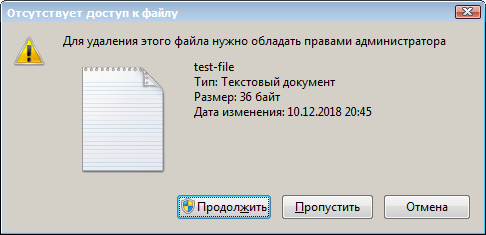
\includegraphics[height = 9\baselineskip]{../01-solution/y03s01-pcdiag-lab-08-p19.png}
				\caption{Вікно попередження при спробі користувача~«\textenglish{user-04}» видалити файл~«\textenglish{test-file}»}
				\label{fig:dir-deletion-attempt-message}
			\end{figure}

			Входимо до системи від імені адміністратора і переглядаємо журнал безпеки. Для цього відкриваємо оснастку «Управління комп'ютером» і обираємо пункт «Перегляд подій». Знаходимо у журналі подію про відмову видалити файл з папки~«\textenglish{Test}» та переглядаємо її~(рис.~\ref{fig:dir-deletion-audit-event}).

			\begin{figure}[!htbp]
				\centering
				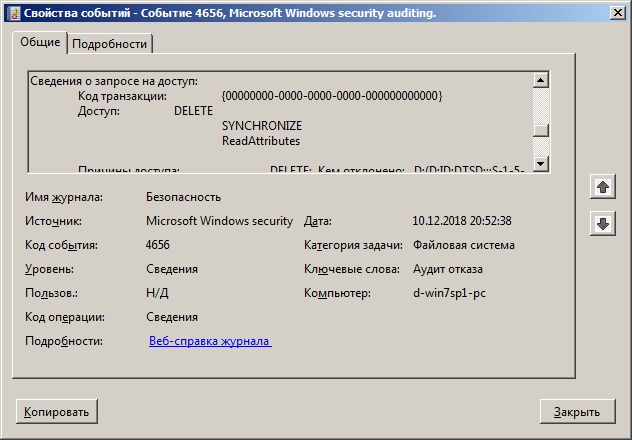
\includegraphics[height = 14\baselineskip]{../01-solution/y03s01-pcdiag-lab-08-p20.png}
				\caption{Деталі події аудиту відмови при спробі користувача~«\textenglish{user-04}» видалити файл~«\textenglish{test-file}»}
				\label{fig:dir-deletion-audit-event}
			\end{figure}

	\section{Висновки}
		Виконуючи дану лабораторну роботу, ми отримали навички адміністрування в~операційній системі~\textenglish{Windows 7}.

\end{document}
